\section{Power budget essentials}

\textbf{Power budget is very tight}. Be careful when sending telecommands! Some telecommands used incorrectly may lead to the end of the mission. First, calculate an impact on the power budget and then test all the telecommand sets on flatsat.

\subsection{Power budget calculations}
Power budget can be considered in two ways: energy in watt hours (Wh) harvested/consumed per orbit or available/consumed mean power. Both approaches can be useful in calculations, depending on feature. For short-term or single events watt hours (Wh) are very useful. For periodic or permanent events mean power will be useful.

Each telecommand with high impact on the power budget have an extended description of the impact on the power budget.

\section{Common concepts}
PW-Sat2 harvests a certain amount of energy per orbit which takes about 98 minutes. During this time the spacecraft is illuminated for about $\frac{2}{3}$ of this time. It consumes some part of this energy to maintain basic functions. It is possible to calculate the excess of energy during this orbit which is available for experiments. It can be converted into mean power also.

A mean power drawn by the spacecraft to maintain basic functions was measured directly. During this measurement the spacecraft was waiting for telecommands and there was no experiment running. System sate:
\begin{itemize}
	\item COMM is waiting for telecommands - receiver is permanently enabled,
	\item OBC is working normally (FRAM, Flash and RTC are working also),
	\item OBC triggers beacons in every 60 s with 1200 bps,
	\item Tumbling lower than 1\textdegree/s on all axes.
\end{itemize}

\subsection{Energy per orbit concept}
MPPT regulators harvest about 2 Wh per orbit. Bus consumes about 1.08 Wh for basic functions. Including both li-ion charging efficiency and DCDC converting efficiency, battery pack will be charged with about 0.5 Wh. So this excess energy can be consumed by experiments. For safety reasons it should be derated.

With this excess of energy the full recharge cycle of the battery pack (about 30 Wh) should take between 4 to 5 days. If it occurs, the spacecraft may be unresponsive for a few days.

\begin{center}
	\begin{tabular}{c|c}
		&[Wh] \\ \hline
		Harvested energy per orbit & 2 \\ \hline
		Energy consumed by basic functions per orbit & 1.08 \\ \hline
		Excess of energy per orbit & 0.5 \\ \hline
		Available energy per orbit for experiments with a margin & \textbf{0.25}
	\end{tabular}
\end{center}

Figure \ref{fig:pwr:energy} shows harvested energy per orbit and energy needed to maintain basic functions.

\begin{figure}[ht]
	\begin{center}
		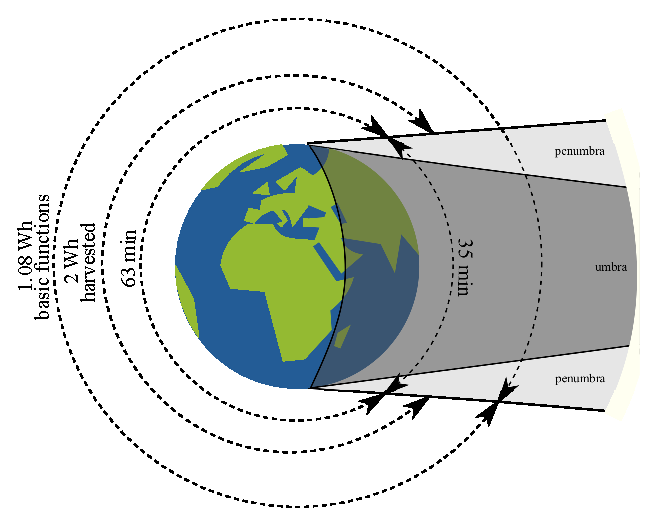
\includegraphics{img/power-budget-energy}
		\caption{Harvested energy and consumed energy by basic functions per orbit}
		\label{fig:pwr:energy}
	\end{center}
\end{figure}

\subsection{Mean power concept}
The harvested energy can be converted into a mean continuous power generated by a hypothetical solar panel. From this power we can subtract a mean power consumption by basic functions. Then mean available power for experiments can be calculated.

\begin{center}
	\begin{tabular}{c|c}
		&[W] \\ \hline
		Mean continuous power generated by a hypothetical solar panel & 1.2 \\ \hline
		Mean power consumption by basic functions & 0.66 \\ \hline
		Excess of mean power & 0.3 \\ \hline
		Available mean power for experiments with a margin & \textbf{0.15}
	\end{tabular}
\end{center}

This is the mean power drawn when no experiment is running. If any experiment is running, then an additional power will be consumed. It depends on experiment what actual mean power is consumed. More data about power consumption of experiments was included in the \texttt{Telecommands} chapter. This additional power should be included in power budget calculations.

\begin{figure}[ht]
	\begin{center}
		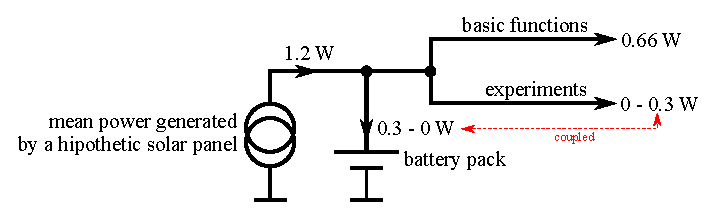
\includegraphics{img/power-budget-power}
		\caption{Power budget based on mean power concept}
		\label{fig:pwr:power}
	\end{center}
\end{figure}

